\documentclass{standalone}
\usepackage{tikz}
\usetikzlibrary{patterns, positioning}
\usepackage[sfdefault]{ClearSans} %% option 'sfdefault' activates Clear Sans as the default text font
\usepackage[T1]{fontenc}

\begin{document}
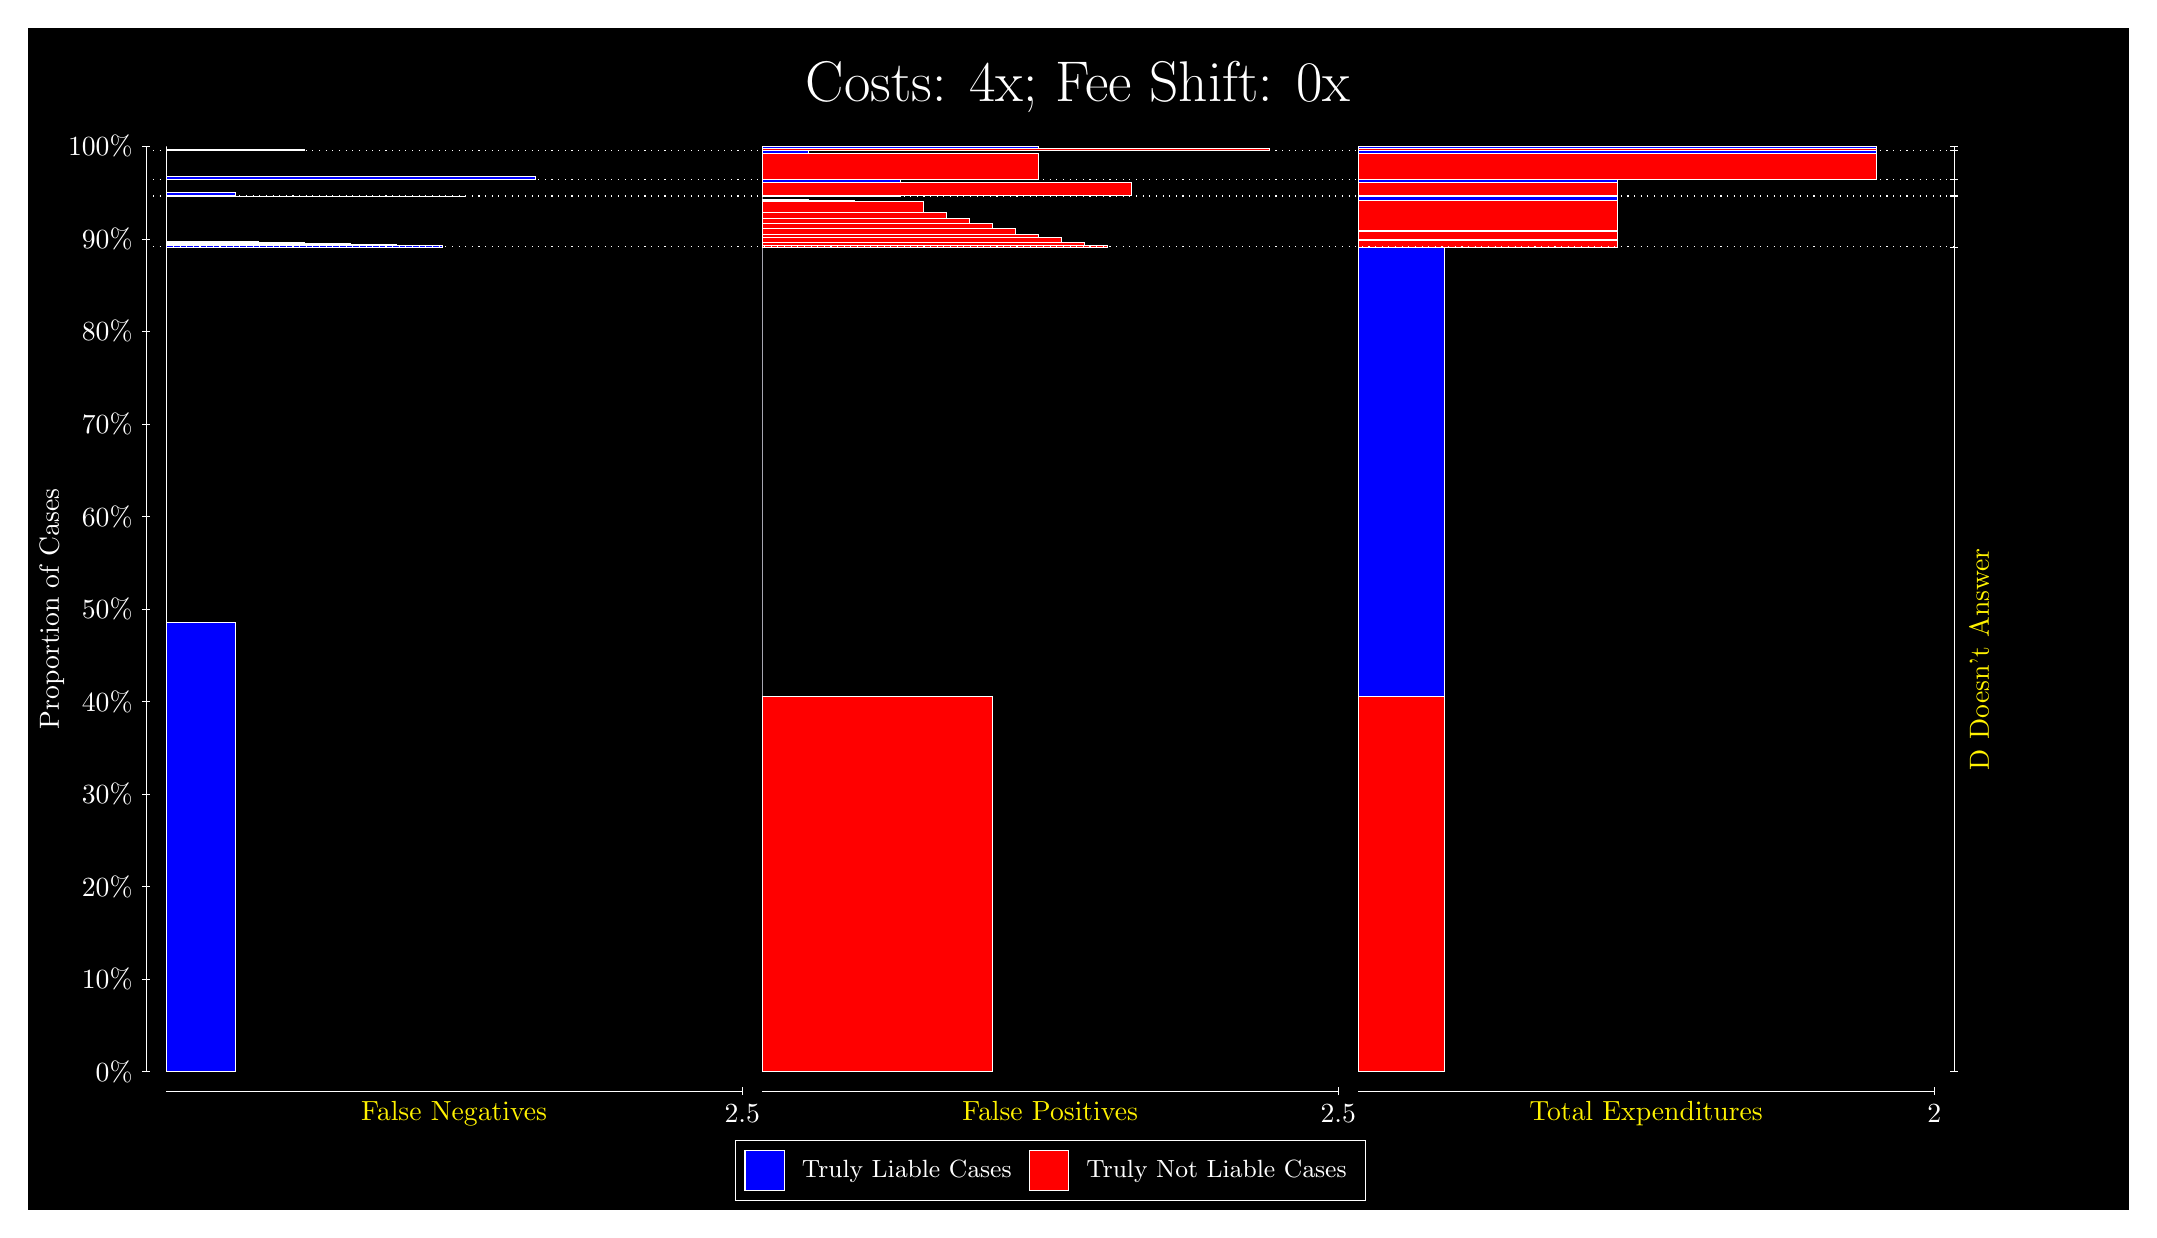
\begin{tikzpicture}
\draw[fill=black] (0,0) rectangle (26.667,15);
\draw[text=white] (0,13.5) rectangle (26.667,15) node[midway] {\huge Costs: 4x; Fee Shift: 0x};
\draw[white, very thin] (1.5,1.75) -- (1.5,13.5);
\node[rotate=90, text=white, anchor=center] at (0.3, 7.625) {Proportion of Cases};
\draw[white, very thin] (1.45,1.75) -- (1.55,1.75);
\node[text=white, anchor=east] at (1.45, 1.75) {0\%};
\draw[white, very thin] (1.45,2.925) -- (1.55,2.925);
\node[text=white, anchor=east] at (1.45, 2.925) {10\%};
\draw[white, very thin] (1.45,4.1) -- (1.55,4.1);
\node[text=white, anchor=east] at (1.45, 4.1) {20\%};
\draw[white, very thin] (1.45,5.275) -- (1.55,5.275);
\node[text=white, anchor=east] at (1.45, 5.275) {30\%};
\draw[white, very thin] (1.45,6.45) -- (1.55,6.45);
\node[text=white, anchor=east] at (1.45, 6.45) {40\%};
\draw[white, very thin] (1.45,7.625) -- (1.55,7.625);
\node[text=white, anchor=east] at (1.45, 7.625) {50\%};
\draw[white, very thin] (1.45,8.8) -- (1.55,8.8);
\node[text=white, anchor=east] at (1.45, 8.8) {60\%};
\draw[white, very thin] (1.45,9.975) -- (1.55,9.975);
\node[text=white, anchor=east] at (1.45, 9.975) {70\%};
\draw[white, very thin] (1.45,11.15) -- (1.55,11.15);
\node[text=white, anchor=east] at (1.45, 11.15) {80\%};
\draw[white, very thin] (1.45,12.325) -- (1.55,12.325);
\node[text=white, anchor=east] at (1.45, 12.325) {90\%};
\draw[white, very thin] (1.45,13.5) -- (1.55,13.5);
\node[text=white, anchor=east] at (1.45, 13.5) {100\%};

\draw[white, very thin] (24.457,1.75) -- (24.457,13.5);
\draw[white, very thin] (24.407,1.75) -- (24.507,1.75);
\node[anchor=west] at (24.407, 1.75) {};
\draw[white, very thin] (24.407,12.224) -- (24.507,12.224);
\node[anchor=west] at (24.407, 12.224) {};
\draw[white, very thin] (24.407,12.866) -- (24.507,12.866);
\node[anchor=west] at (24.407, 12.866) {};
\draw[white, very thin] (24.407,12.88) -- (24.507,12.88);
\node[anchor=west] at (24.407, 12.88) {};
\draw[white, very thin] (24.407,13.084) -- (24.507,13.084);
\node[anchor=west] at (24.407, 13.084) {};
\draw[white, very thin] (24.407,13.444) -- (24.507,13.444);
\node[anchor=west] at (24.407, 13.444) {};
\draw[white, very thin] (24.407,13.5) -- (24.507,13.5);
\node[anchor=west] at (24.407, 13.5) {};

\draw[white, very thin, fill=blue] (1.75,1.75) rectangle (2.6283,7.4593);
\draw[white, very thin, fill=red] (1.75,7.4593) rectangle (1.75,12.224);
\draw[white, very thin, fill=blue] (1.75,12.224) rectangle (5.2631,12.238);
\draw[white, very thin, fill=blue] (1.75,12.238) rectangle (4.9703,12.245);
\draw[white, very thin, fill=blue] (1.75,12.245) rectangle (4.6775,12.252);
\draw[white, very thin, fill=blue] (1.75,12.252) rectangle (4.3848,12.256);
\draw[white, very thin, fill=blue] (1.75,12.256) rectangle (4.3848,12.258);
\draw[white, very thin, fill=blue] (1.75,12.258) rectangle (4.092,12.266);
\draw[white, very thin, fill=blue] (1.75,12.266) rectangle (3.7993,12.27);
\draw[white, very thin, fill=blue] (1.75,12.27) rectangle (3.5065,12.278);
\draw[white, very thin, fill=blue] (1.75,12.278) rectangle (3.2138,12.284);
\draw[white, very thin, fill=blue] (1.75,12.284) rectangle (2.921,12.291);
\draw[white, very thin, fill=red] (1.75,12.291) rectangle (1.75,12.866);
\draw[white, very thin, fill=blue] (1.75,12.866) rectangle (5.5558,12.867);
\draw[white, very thin, fill=red] (1.75,12.867) rectangle (1.75,12.88);
\draw[white, very thin, fill=blue] (1.75,12.88) rectangle (2.6283,12.92);
\draw[white, very thin, fill=red] (1.75,12.92) rectangle (1.75,13.084);
\draw[white, very thin, fill=blue] (1.75,13.084) rectangle (6.4341,13.121);
\draw[white, very thin, fill=red] (1.75,13.121) rectangle (1.75,13.444);
\draw[white, very thin, fill=blue] (1.75,13.444) rectangle (3.5065,13.464);
\draw[white, very thin, fill=red] (1.75,13.464) rectangle (1.75,13.5);
\draw[white, very thin, fill=red] (9.3189,1.75) rectangle (12.246,6.5147);
\draw[white, very thin, fill=blue] (9.3189,6.5147) rectangle (9.3189,12.224);
\draw[white, very thin, fill=red] (9.3189,12.224) rectangle (13.71,12.249);
\draw[white, very thin, fill=red] (9.3189,12.249) rectangle (13.417,12.287);
\draw[white, very thin, fill=red] (9.3189,12.287) rectangle (13.125,12.346);
\draw[white, very thin, fill=red] (9.3189,12.346) rectangle (12.832,12.384);
\draw[white, very thin, fill=red] (9.3189,12.384) rectangle (12.539,12.465);
\draw[white, very thin, fill=red] (9.3189,12.465) rectangle (12.246,12.524);
\draw[white, very thin, fill=red] (9.3189,12.524) rectangle (11.954,12.592);
\draw[white, very thin, fill=red] (9.3189,12.592) rectangle (11.661,12.662);
\draw[white, very thin, fill=red] (9.3189,12.662) rectangle (11.368,12.799);
\draw[white, very thin, fill=blue] (9.3189,12.799) rectangle (10.783,12.806);
\draw[white, very thin, fill=blue] (9.3189,12.806) rectangle (10.49,12.812);
\draw[white, very thin, fill=blue] (9.3189,12.812) rectangle (10.197,12.82);
\draw[white, very thin, fill=blue] (9.3189,12.82) rectangle (9.9044,12.824);
\draw[white, very thin, fill=blue] (9.3189,12.824) rectangle (9.6116,12.832);
\draw[white, very thin, fill=blue] (9.3189,12.832) rectangle (9.3189,12.866);
\draw[white, very thin, fill=red] (9.3189,12.866) rectangle (11.075,12.879);
\draw[white, very thin, fill=blue] (9.3189,12.879) rectangle (9.3189,12.88);
\draw[white, very thin, fill=red] (9.3189,12.88) rectangle (14.003,13.043);
\draw[white, very thin, fill=blue] (9.3189,13.043) rectangle (11.075,13.084);
\draw[white, very thin, fill=red] (9.3189,13.084) rectangle (12.832,13.407);
\draw[white, very thin, fill=blue] (9.3189,13.407) rectangle (9.9044,13.444);
\draw[white, very thin, fill=red] (9.3189,13.444) rectangle (15.759,13.48);
\draw[white, very thin, fill=blue] (9.3189,13.48) rectangle (12.832,13.5);
\draw[white, very thin, fill=red] (16.888,1.75) rectangle (17.986,6.5147);
\draw[white, very thin, fill=blue] (16.888,6.5147) rectangle (17.986,12.224);
\draw[white, very thin, fill=red] (16.888,12.224) rectangle (20.181,12.305);
\draw[white, very thin, fill=blue] (16.888,12.305) rectangle (20.181,12.314);
\draw[white, very thin, fill=red] (16.888,12.314) rectangle (20.181,12.427);
\draw[white, very thin, fill=blue] (16.888,12.427) rectangle (20.181,12.438);
\draw[white, very thin, fill=red] (16.888,12.438) rectangle (20.181,12.819);
\draw[white, very thin, fill=blue] (16.888,12.819) rectangle (20.181,12.866);
\draw[white, very thin, fill=red] (16.888,12.866) rectangle (20.181,12.879);
\draw[white, very thin, fill=blue] (16.888,12.879) rectangle (20.181,12.88);
\draw[white, very thin, fill=red] (16.888,12.88) rectangle (20.181,13.043);
\draw[white, very thin, fill=blue] (16.888,13.043) rectangle (20.181,13.084);
\draw[white, very thin, fill=red] (16.888,13.084) rectangle (23.475,13.407);
\draw[white, very thin, fill=blue] (16.888,13.407) rectangle (23.475,13.444);
\draw[white, very thin, fill=red] (16.888,13.444) rectangle (23.475,13.48);
\draw[white, very thin, fill=blue] (16.888,13.48) rectangle (23.475,13.5);
\draw[white, dotted] (1.5,12.224) -- (24.457,12.224);
\draw[white, dotted] (1.5,12.866) -- (24.457,12.866);
\draw[white, dotted] (1.5,12.88) -- (24.457,12.88);
\draw[white, dotted] (1.5,13.084) -- (24.457,13.084);
\draw[white, dotted] (1.5,13.444) -- (24.457,13.444);
\draw[white, very thin] (1.75,1.5) -- (9.0689,1.5);
\node[text=yellow, anchor=north] at (5.4094, 1.5) {False Negatives};
\draw[white, very thin] (9.0689,1.45) -- (9.0689,1.55);
\node[text=white, anchor=north] at (9.0689, 1.45) {2.5};

\draw[white, very thin] (9.3189,1.5) -- (16.638,1.5);
\node[text=yellow, anchor=north] at (12.978, 1.5) {False Positives};
\draw[white, very thin] (16.638,1.45) -- (16.638,1.55);
\node[text=white, anchor=north] at (16.638, 1.45) {2.5};

\draw[white, very thin] (16.888,1.5) -- (24.207,1.5);
\node[text=yellow, anchor=north] at (20.547, 1.5) {Total Expenditures};
\draw[white, very thin] (24.207,1.45) -- (24.207,1.55);
\node[text=white, anchor=north] at (24.207, 1.45) {2};

\node[text=yellow, centered, rotate=90] at (24.777, 6.987) {D Doesn't Answer};






\draw (12.978300999999998,1.5) node[draw=none] (baseCoordinate) {};
\begin{scope}[align=center]
        \matrix[scale=0.5, draw=white, below=0.5cm of baseCoordinate, nodes={draw}, column sep=0.1cm]{
            \node[rectangle, draw, minimum width=0.5cm, minimum height=0.5cm, fill=blue] {}; &
            \node[draw=none, font=\small, text=white] (B) {Truly Liable Cases}; &
            \node[rectangle, draw, minimum width=0.5cm, minimum height=0.5cm, fill=red] {}; &
            \node[draw=none, font=\small, text=white] (B) {Truly Not Liable Cases}; \\
            };
\end{scope}

\end{tikzpicture}
\end{document}